\section{Resultados}
\label{sec:resultados}

A implantação do sistema descrito nas seções anteriores é, de certa maneira, hierárquica: para que um subssistema de alto-nível funcione, os que estão abaixo dele devem estar funcionando também. Tal conceito pode ser visto na Figura \ref{fig:sistema} Portanto, os testes e validações ocorreram de maneira concomitante ao desenvolvimento do software e montagem da estrutura.

Devido ao fato do computador não ser um sistema 100\% apropriado para tempo real balbalbalbalbabalalbal a tmeporização dos sensores fic preocupante. ASsim, s emediu as leituras obtidas para cada encoder, e se obteve o seguinte, comforme  aFIgura \ref{fig:pos_encoder}.

\begin{figure}[h]
  \centering
  
\includegraphics[width = 0.3\textwidth]{imagens/edc}
  \caption{Encoderdoderdoder.}
  \label{fig:pos_encoder}
\end{figure}

Durante os testes de acionamento dos motores, se percebeu uma não linearidade do tipo ``zona-morta'', e foi realizado um ensaio para quantificar o problema. Os resultados de tal ensaio podem ser vistos na Figura \ref{fig:zonamorta}. Foi implementado um controlador proporcional para a velocidade, com ganho bastante baixo, de modo a tornar a resposta do sistema lenta, e foram definidos \emph{setpoints} que propositalmente levassem a saturação dos \textit{drivers} dos atuadores. Na Figura, se pode enxergar a zona morta em torno de $t=$1.5 s, quando a velocidade da roda se eleva repentinamente, e entre $t=$ 4 s e $t=$ 5 s, quando foi realizado o comando de inversão da velocidade da roda, e para um intervalo de valores de acionamento em torno da origem, não há movimento no eixo. Esta não linearidade é oriunda do atrito estático introduzido pelos componentes mecânicos responsáveis pela relação de redução. \textit{tenho mais um gráfico mostrando q dá pra andar bem devagar se já estiver andando no inicio... temos espaço??}

\begin{figure}[h]
  \centering
  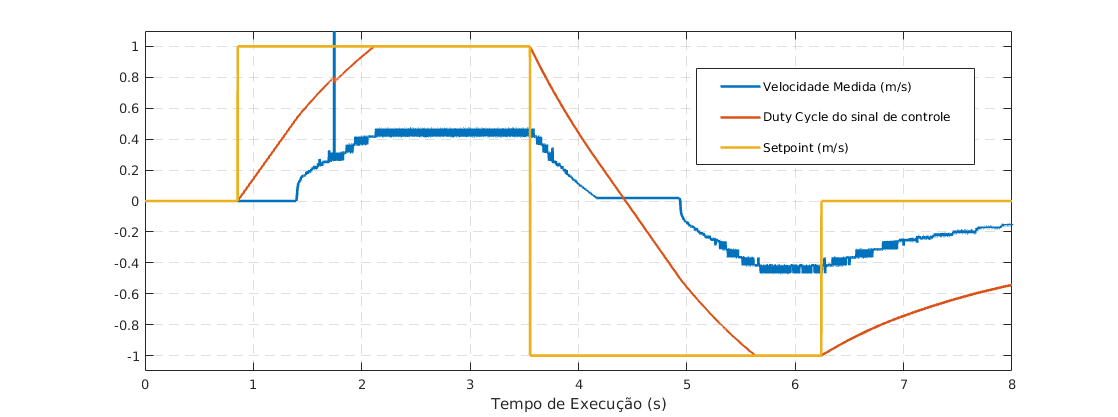
\includegraphics[width = \textwidth]{imagens/zonamorta}
  \caption{Análise da não-linearidade do tipo ``zona-morta'' presente nos motores utilizados.}
  \label{fig:zonamorta}
\end{figure}

O ensaio foi realizado simultaneamente com as três rodas, e como todas as leituras apresentaram resultados similares, apenas uma aparece no gráfico.

Uma consequência deste efeito foi verificada no acionamento do robô em trajetórias que exigem baixas velocidades de alguma das rodas. Esta situação pode ser vista na Figura \ref{fig:zm3rodas}. Na figura, se pode ver como os motores que devem operar em velocidades menores entram em operação mais tarde, causando desvios de trajetória. \textit{tenho mais um monte de dados parecidos, para varias velocidades e vários ganhos}

\begin{figure}[h]
  \centering
  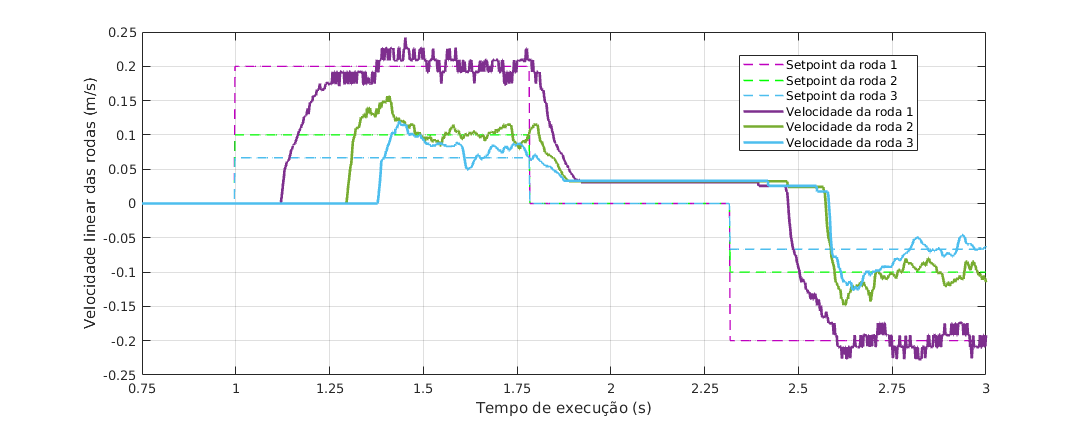
\includegraphics[width = \textwidth]{imagens/zm3rodas}
  \caption{Efeito da zona morta no acionamento das 3 rodas com velocidades distintas.}
  \label{fig:zm3rodas}
\end{figure}

(está com velocidades bem baixinhas, se estiver um pouco mais rápido melhora)

\cite{cunha2001zm} propõe um jeito de se resolver isso. Aplicando esse jeito, se conseguiram melhorar bastante os resultaos, veja na FIgura \ref{fig:zm_comp}, logo abaix alskdjhalksjdhlaskdjhal.

\begin{figure}[h]
  \centering
  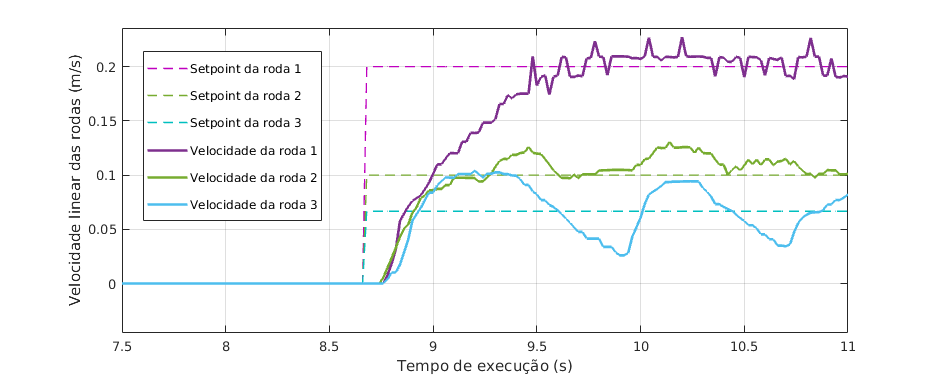
\includegraphics[width = \textwidth]{imagens/zmcomp}
  \caption{Não linearidade compensada, mostrando o acionamento quase simultâneo de todas as rodas.}
  \label{fig:zm_comp}
\end{figure}

Desvio padrão do tmepo de execução do loop: 16,68573853

Tempo médio a cada chamada do loop de controle, em $\mu$s: 10000,03822

resultados do controle de velocidade

\begin{figure}[h]
  \centering
  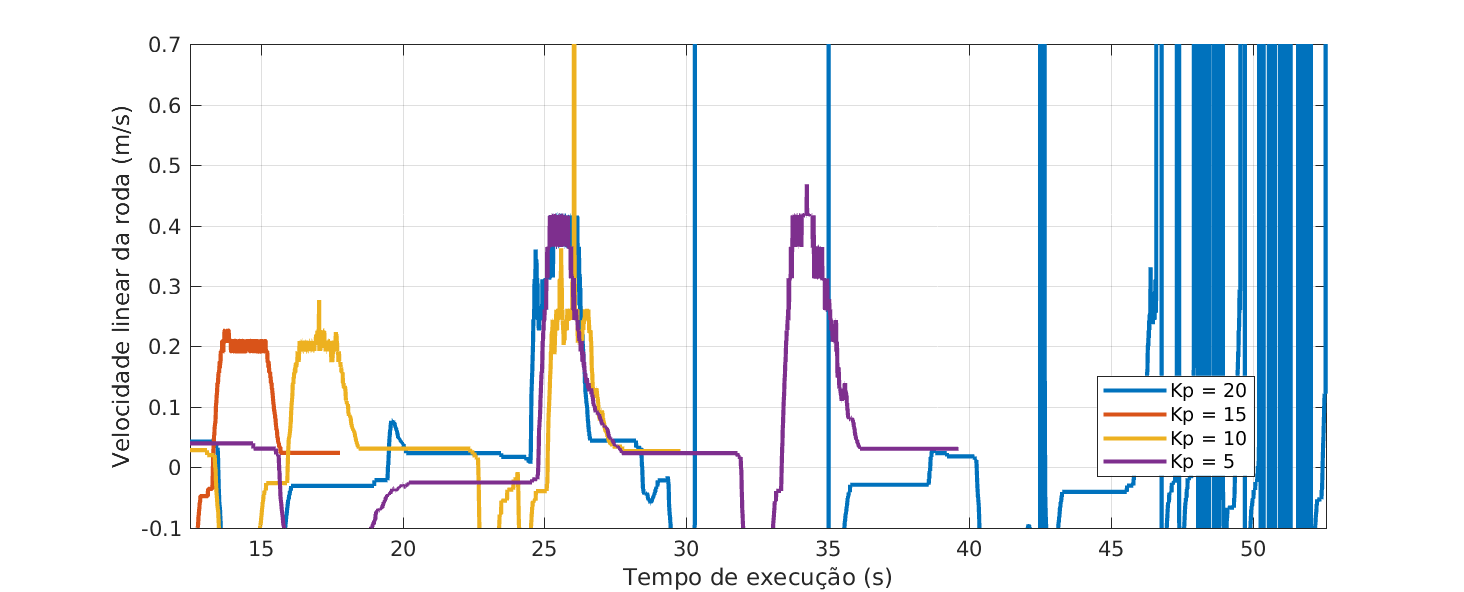
\includegraphics[width = \textwidth]{imagens/inst}
  \caption{Resultados de operação aleatória do robô utilizando ganhos arbitrários.}
  \label{fig:inst}
\end{figure}

resultados da calibração da velocidade, com fator de conversão 480 ao invés de 534.
0.1, 0.2, 0.4
\citet{lynch2017modern}: In most robotic applications, higher control update rates are of limited benefit, given
time constants associated with the dynamics of the robot and environment.

resultados da odometria:
Growth of the pose uncertainty for straight-line movement: Note that the uncertainty in y grows much
faster than in the direction of movement. This results from the integration of the uncertainty about the
robot’s orientation. \citep{siegwart2011introduction}

resultados do controle de posição

tempo de duração da bateria
